\chapter{Jednoduchý regresní model}

\section{Definice regresního modelu}

Jednoduchý regresní model populace je definován rovnicí
\begin{equation}
y = \beta_0 + \beta_1 x + u,
\end{equation}
kde $y$ představuje závislou (vysvětlovanou) veličinu, $x$ nezávislou (vysvětlující) veličinu a $u$ je tzv. 
chybová složka reprezentující faktory, které nejsou zahrnuty v $x$ a které mající vliv na $y$. Parametr $\beta_0$ nazýváme 
průsečíkem regresního modelu a parametr $\beta_1$ je pak sklonem regresního modelu vzhledem k nezávislé veličině $x$. Jestliže jsou ostatní faktory 
reprezentované členem $u$ konstantní, tj. $\Delta u = 0$, pak je vztah mezi $x$ a $y$ lineární.
\begin{equation}
\Delta y = \beta_1 \Delta x
\end{equation}
(2.2) implicitně předpokládá, že $E[u] = 0$. Tento předpoklad však ve skutečnosti není 
omezující, protože je vždy možné upravit parametr $\beta_0$ tak, aby $E[u] = 0$. Zásadnějším předpokladem 
je $E[u|x] = E[u] = 0$, tj. předpoklad, že chyba $u$ a vysvětlující veličina $x$ jsou nezávislé. Rovnice $E[u|x] = 0$ říká, že 
průměrná hodnota chyby $u$ je nulová napříč všemi podvýběry definovanými konkrétní hodnotou vysvětlující veličiny
$x$\footnote{Uvažujme ekonometrický model, kde $y$ představuje výnos na hektar, $x$ kvalitu půdy a $u$ zahrnuje 
množství hnojiv, které jsme použili. Pokud bude množství hnojiv nezávislé na kvalitě půdy, pak je předpoklad 
$E[u|x] = E[x] = 0$ splněn. Pokud však použijeme více hnojiva na méně kvalitní půdu, je tento předpoklad porušen.}.

Očekávaná hodnota (2.1) je daná tzv. populační regresní funkcí (population regression function - PRF)
\begin{equation}
E[y|x] = \beta_0 + \beta_1 x,
\end{equation}
kde pravděpodobnostní rozdělení veličiny $y$ je centrováno na $E[y|x]$ pro libovolnou hodnotu $x$. Situace je 
ilustrována následujícím obrázkem.

\begin{figure}[htp]
\centering
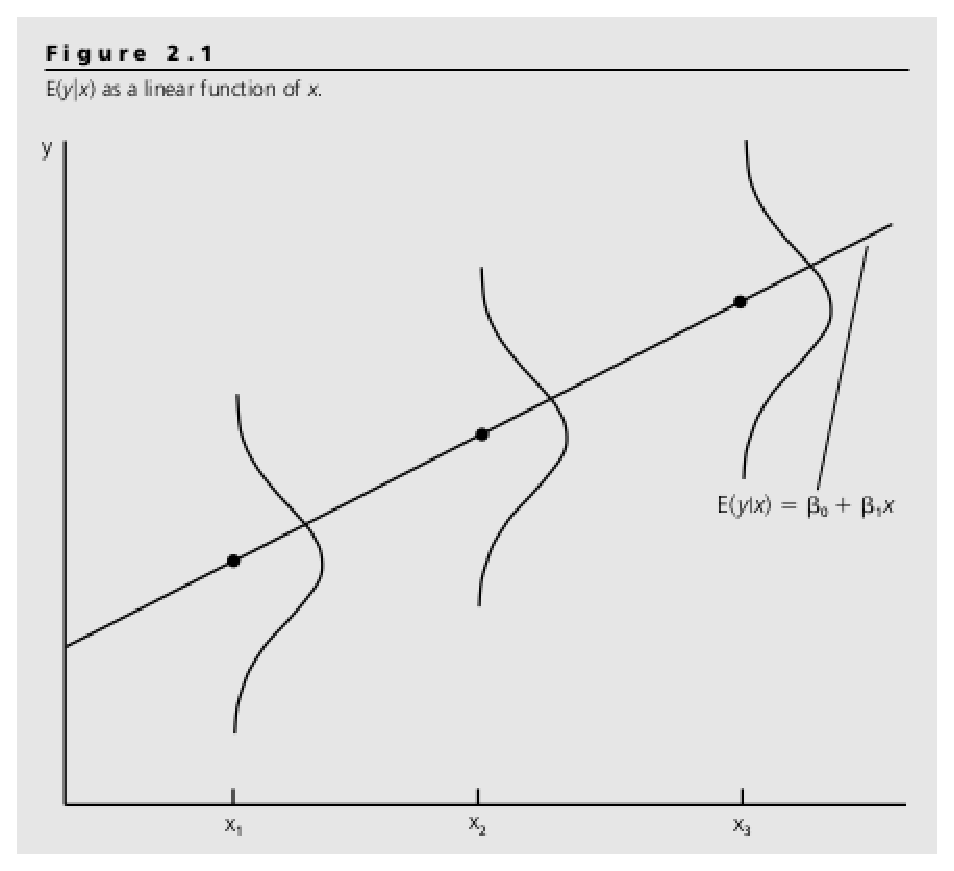
\includegraphics[scale = 0.5]{pictures/figure_2_1.eps}
\caption{$E[y|x]$ jako lineární funkce $x$}
\label{figure_2_1}
\end{figure} 

S ohledem na $E[u|x] = 0$ je užitečné (2.1) rozdělit na dvě části. Část $\beta_0 + \beta_1 x$ reprezentující $E[y|x]$ je nazývána systematickou částí $y$, tj. částí vysvětlenou nezávislou proměnnou $x$; část $u$ je 
nazývána nesystematickou částí, tj. částí $y$, která není vysvětlená nezávislou proměnnou $x$.

\section{Metoda nejmenších čtverců}

Uvažujme jednoduchý regresní model
\begin{equation}
y_i = \beta_0 + \beta_1 x_i + u_i.
\end{equation}
Protože $E[u|x] = E[u] = 0$ implikuje nezávislost $x$ a $u$, platí
\begin{equation}
cov(x,u) = E[ux] - E[x]E[y] = E[ux] = 0.
\end{equation}
Rovnice $E[u] = 0$ a $E[xy] = 0$ lze přepsat do tvaru
\begin{equation}
E[y - \beta_0 - \beta_1 x] = 0
\end{equation}
a
\begin{equation}
E[x(y - \beta_0 - \beta_1 x)] = 0.
\end{equation}
Odhady parametrů $\hat{\beta}_0$ a $\hat{\beta}_1$ jsou řešením soustavy rovnic
\begin{equation}
n^{-1} \sum_{i = 1}^n (y_i - \hat{\beta}_0 - \hat{\beta}_1x_i) = 0
\end{equation}
a
\begin{equation}
n^{-1} \sum_{i = 1}^n x_i (y_i - \hat{\beta}_0 - \hat{\beta}_1x_i) = 0.
\end{equation}
Protože $\bar{y} = \hat{\beta}_0 + \hat{\beta}_1 \bar{x}$, tj.
\begin{equation}
\hat{\beta}_0 = \bar{y} - \hat{\beta}_1 \bar{x},
\end{equation}
lze rovnici (2.9) postupně upravit následujícím způsobem.
\begin{equation}
\sum_{i = 1}^n x_i(y_i - (\bar{y} - \hat{\beta}_1 \bar{x}) - \hat{\beta}_1x_i) = 0
\end{equation}
\begin{equation}
\sum_{i = 1}^n x_i(y_i - \bar{y}) = \hat{\beta}_1 \sum_{i = 1}^n x_i(x_i - \hat{x})
\end{equation}
S využitím vztahů
\begin{equation}
\sum_{i = 1}^n x_i (x_i - \bar{x}) = \sum_{i = 1}^n (x_i - \bar{x})^2
\end{equation}
a
\begin{equation}
\sum_{i = 1}^n x_i(y_i - \bar{y}) = \sum_{i = 1}^n (x_i - \bar{x})(y_i - \bar{y})
\end{equation}
lze $\hat{\beta}_1$ vyjádřit jako
\begin{equation}
\hat{\beta}_1 = \frac{\sum_{i = 1}^n (x_i - \bar{x})(y_i - \bar{y})}{\sum_{i = 1}^n (x_i - \bar{x})^2},
\end{equation}
Pokud čitatel i jmenovatel (2.15) vydělíme $n - 1$, lze odhad $\hat{\beta}_1$ interpretovat jako podíl kovariance mezi $x$ a $y$ a výběrového rozptylu $x$. Odhady (2.10) a (2.15) se nazývají odhady nejmenších čtverců 
(ordinary least square estimates - OLS estimates).

Rovnici hodnot odhadnutých na základě regresního modelu, označovanou jako OLS regresní přímka popř. jako 
výběrovou regresní funkci (sample regression function - SRF), zapisujeme ve tvaru
\begin{equation}
\hat{y}_i = \hat{\beta}_0 + \hat{\beta}_ix_1
\end{equation}
a rovnici reziduí jednotlivých pozorování\footnote{Člen $u$ populačního regresního modelu $y = \beta_0 + 
\beta_1 x + u$ označujeme jako chybu. Člen $\hat{u}$ odhadu populačního regresního modelu $y = \hat{\beta}_0 + 
\hat{\beta}_1 x + \hat{u}$ pak označujeme jako reziduum.} pak jako
\begin{equation}
\hat{u}_i = y_i - \hat{y}_i = y_i - \hat{\beta}_0 - \hat{\beta}_1x_i.
\end{equation}
Jestliže parciální derivace součtu čtverců reziduí
\begin{equation}
\sum_{i = 1}^n \hat{u}_i^2 = \sum_{i = 1}^n (y_i - \hat{\beta}_0 - \hat{\beta}_1 x_1)^2
\end{equation}
dle $\hat{\beta}_0$ a $\hat{\beta}_1$ položíme rovny nule a řešíme pro $\hat{\beta}_0$ a $\hat{\beta}_1$, 
získáme (2.10) a (2.15). Jinými slovy (2.10) a (2.15) minimalizují (2.18) - odtud pojem metoda nejmenších čtverců.

\section{Vlastnosti OLS pro náhodný výběr}

Následující tvrzení implicitně předpokládají, že odhad regresního modelu je proveden na náhodném výběru z populace, kterou zamýšlíme 
tímto modelem popsat.

\subsection{Algebraické vlastnosti OLS}

Průměr reziduí $\hat{u}_i = y_i - \hat{\beta}_0 - \hat{\beta}_1x_1$ je roven nule, tj.
\begin{equation}
\sum_{i = 1}^n \hat{u}_i = 0.
\end{equation}
Toto tvrzení je přímým důsledkem toho, jakým způsobem jsou zkonstruovány odhady $\hat{\beta}_0$ a 
$\hat{\beta}_1$.

Vztah (2.19) implikuje nulovou OLS kovarianci, tj.
\begin{equation}
\sum_{i = 1}^n x_i \hat{u}_i = 0.
\end{equation}

Bod $(\bar{x}, \bar{y})$ se vždy nachází na OLS regresní přímce. Toto tvrzení vyplývá z (2.10).

Na OLS lze pohlížet jako na metodu, která rozdělí pozorování $y_i$ na $\hat{y}_i = \hat{\beta}_0 + 
\hat{\beta}_1x_1$ predikované OLS přímkou a rezidua $\hat{u}_i = y_i - \hat{y}_i$. Rezidua $\hat{u}_i$ a 
predikované hodnoty $\hat{y}_i$ jsou v rámci náhodného výběru nekorelované.

Definujme celkový součet čtverců (total sum of squares - SST), vysvětlený součet čtverců (explained sum of 
squares - SSE) a reziduální součet čtverců (residual sum of squares - SSR) jako
\begin{equation}
SST \equiv \sum_{i = 1}^n (y_i - \bar{y})^2,
\end{equation}
\begin{equation}
SSE \equiv \sum_{i = 1}^n (\hat{y}_i - \bar{y})^2,
\end{equation}
a
\begin{equation}
SSR \equiv \sum_{i = 1}^n \hat{u}_i^2.
\end{equation}
Platí
\begin{equation}
SST = SSE + SSR.
\end{equation}
To lze dokázat následujícím způsobem s využitím $\sum_{i = 1}^n \hat{u}_i(\hat{y}_i - \bar{y}) = 0$, což je 
ekvivalentní předpokladu nulové výběrové kovariance mezi rezidui $\hat{u}_i$ a predikovanými hodnotami $\hat{y}_i$.
\begin{equation}
\begin{split}
SST = \sum_{i = 1}^n (y_i - \bar{y})^2 & = \sum_{i = 1}^n [(y_i - \hat{y}_i) + (\hat{y}_i + \bar{y})]^2\\
& = \sum_{i = 1}^n [\hat{u}_i + (\hat{y}_i - \bar{y})]^2\\
& = \sum_{i = 1}^n \hat{u}_i^2 + 2 \sum_{i = 1}^n \hat{u}_i(\hat{y}_i - \bar{y}) + \sum_{i = 1}^n (\hat{y}_i - 
\bar{y})^2\\
& = SSR + SSE
\end{split}
\end{equation}

\subsection{Míra shody (goodness-of-fit)}

Pro vyjádření míry shody mezi pozorovanými a predikovanými hodnotami se v ekonometrii používá tzv. $R^2$, 
někdy též nazývaný koeficient determinace.
\begin{equation}
R^2 = \frac{SSE}{SST} = 1 - \frac{SSR}{SST}.
\end{equation}
Z výše uvedené rovnice vyplývá, že $R^2$ je poměrem mezi vysvětleným a celkovým rozptylem závislé proměnné. 
$R^2$ tak vždy nabývá hodnoty v rozmezí nula až jedna. V případě jednoduchého regresního modelu s jednou 
nezávislou proměnnou je $R^2$ rovno druhé mocnině korelačního koeficientu mezi $y_i$ a $\hat{y}_i$; odtud 
pochází název $R^2$.

V sociálních vědách se velmi často setkáváme s regresními modely, jejichž $R^2$ je poměrně nízké. Zdánlivě 
nízké $R^2$ nemusí nezbytně znamenat, že model je špatný. Takovýto model může stále dobře popisovat 
lineární vztahy mezi vybranými veličinami. Problémem modelu však je, že nezávislá veličina $x$ podchycuje 
pouze menší část variace závislé veličiny $y$.

\section{Měrné jednotky a nelinearity v regresním modelu}

\subsection{Efekt změny měrné jednotky na OLS statistiky}

Jestliže změníme měrné jednotky závislé či nezávislé proměnné, změní se OLS odhady deterministickým způsobem.

Pokud je závislá proměnná $y$ vynásobena konstantou $c$, pak jsou OLS odhady průsečíku $\hat{\beta}_0$ a sklonu 
regresního modelu $\hat{\beta}_1$ taktéž vynásobeny konstantou $c$.

V případě, že je nezávislá veličina $x$ vydělená popř. vynásobena nenulovou konstantou $c$, je odhad sklon 
$\hat{\beta_1}$ této nezávislé veličiny taktéž vynásoben popř. vydělen touto konstantou. Odhad průsečíku $\hat{\beta}_0$ regresního modelu zůstává nezměněn.

Míra shody vyjádřená pomocí $R^2$ je změnou měrné jednotky nedotčena.

\subsection{Zahrnutí nelinearit do regresního modelu}

\subsubsection{Log-level regresní model}

Jednoduchý regresní model $y = \beta_0 + \beta_1 x + u$ označujeme jako level-level model. Jeho 
triviální modifikací je tzv. log-level model
\begin{equation}
ln(y) = \beta_0 + \beta_1 x + u.
\end{equation}
Tento model říká, o kolik procentních bodů se zvýší $y$, jestliže se $x$ zvýší o jednu jednotku. Jinými slovy
\begin{equation}
\%\Delta y \approx (100 \beta_1) \Delta x.
\end{equation}
Veličina $100 \beta_1$ je někdy nazývána semi-elasticitou. Model (2.27) lze upravit do tvaru
\begin{equation}
y = e^{\beta_0 + \beta_1 x + u},
\end{equation}
Takto upravený model je typický exponenciálním průběhem.

\begin{figure}[htp]
\centering
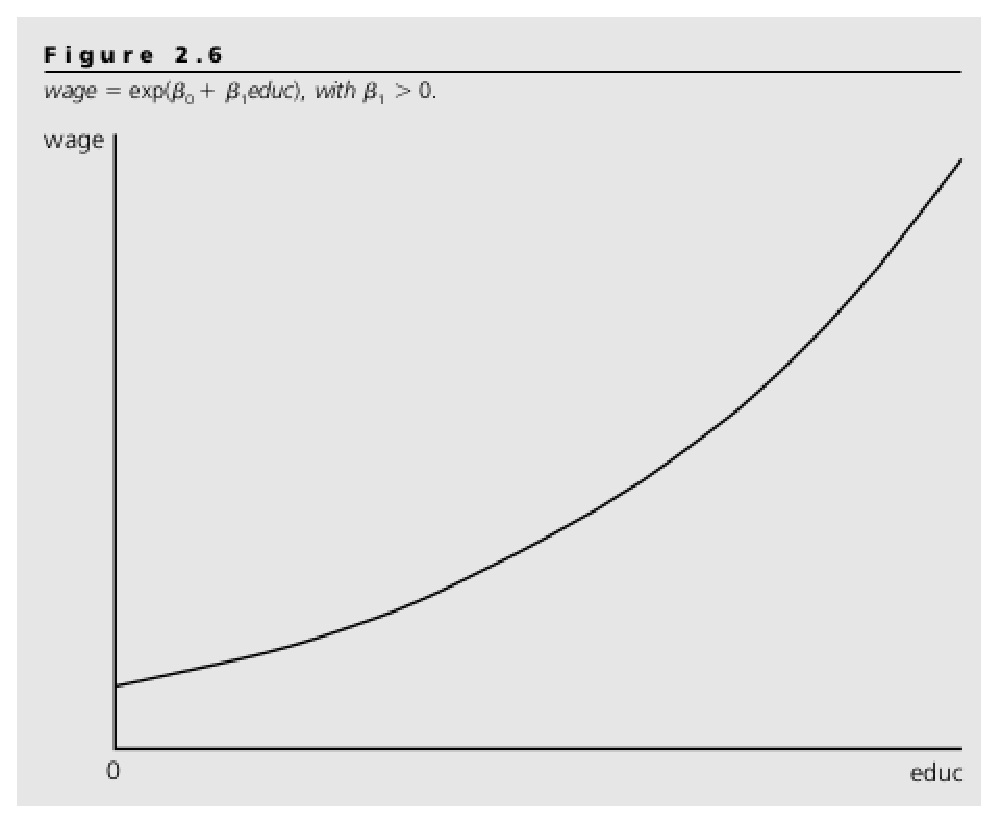
\includegraphics[scale = 0.5]{pictures/figure_2_6.eps}
\caption{Regresní model s exponenciálním průběhem}
\label{figure_2_6}
\end{figure} 

\subsubsection{Log-log regresní model}

Další modifikací základního regresního modelu je tzv. log-log model nazývaný též modelem konstantní elasticity, který má tvar
\begin{equation}
ln(y) = \beta_0 + \beta_1 ln(x) + u.
\end{equation}
Tento model říká, že pokud se $x$ zvýší o 1\%, zvýší se $y$ o $\beta_1$\%, což je obvyklá interpretace elasticity.

\subsubsection{Změna měrné jednotky}

Pokud ve výše uvedených modelech závislou popř. nezávislou proměnnou vynásobíme konstantou $c$, sklon regresního modelu zůstane 
nezměněn, nicméně jeho průsečík se změní na $ln(c) + \beta_0$.

\subsection{Význam pojmu lineární regrese}

Pojem lineární regrese se váže k parametrům modelu, nikoliv k podkladovým datům. Model
\begin{equation}
y = \beta_0 + \beta_1 x^2 + u
\end{equation}
je tak stále lineárním regresním modelem, nicméně model
\begin{equation}
y = \frac{1}{\beta_0 + \beta_1 x + u}
\end{equation}
již lineárním regresním modelem není.

\section{Očekávaná hodnota a rozptyl OLS odhadů}

\subsection{Nestrannost OLS odhadů (unbiasedness of OLS)}

Tuto kapitolu zahájíme souhrnem předpokladů, na základě kterých budeme následně dokazovat nestrannost OLS odhadů.

\begin{assumption}[SLR.1 - lineární model]
V populačním regresním modelu je vztah mezi závislou veličinou $y$ a nezávislou veličinou $x$ a chybou $u$ charakterizován funkcí ve tvaru
\begin{equation}
y = \beta_0 + \beta_1 x + u,
\end{equation}
kde $\beta_0$ a $\beta_1$ jsou populační průsečík a sklon.

\raggedleft{$\clubsuit$}
\end{assumption}

\begin{assumption}[SLR.2 - náhodný výběr]
Máme k dispozici náhodný výběr velikosti $n$, $\{(x_i, y_i): i = 1, 2, ..., n \}$, který sleduje populační model definovaný v předpokladu SLR.1.

\raggedleft{$\clubsuit$}
\end{assumption}

\begin{assumption}[SLR.3 - výběrový rozptyl vysvětlující veličiny]
Náhodně vybrané vysvětlující proměnné $\{x_i, i = 1, 2, ..., n\}$ nenabývají stejné hodnoty. Jinými slovy 
výběrový rozptyl vysvětlující proměnné je různý od nuly.

\raggedleft{$\clubsuit$}
\end{assumption}

\begin{assumption}[SLR.4 - nulová podmíněná hodnota]
Očekávaná hodnota chyby $u$ je pro libovolnou hodnotu závislé veličiny rovna nule, tj.
\begin{equation}
E[u|x] = 0.
\end{equation}

\raggedleft{$\clubsuit$}
\end{assumption}

Skutečný populační sklon $\beta_1$ neznáme, máme však k dispozici jeho odhad - výběrový sklon 
$\hat{\beta}_1$. Ten je náhodnou veličinou, a proto má očekávanou hodnotu a rozptyl.

Protože $\sum_{i = 1}^n (x_i - \bar{x})(y_i - \bar{y}) = \sum_{i = 1}^n (x_i - \bar{x})y_i$, lze $\hat{\beta}_1$ vyjádřit jako
\begin{equation}
\hat{\beta}_1 = \frac{\sum_{i = 1}^n (x_i - \bar{x})y_i}{\sum_{i = 1}^n (x_i - \bar{x})^2}.
\end{equation}
Vzhledem k tomu, že $SST_x = \sum_{i = 1}^n (x_i - \bar{x})^2$ a $y_i = \beta_0 + \beta_1 x_i + u_i$, můžeme výše 
uvedenou rovnici upravit do tvaru
\begin{equation}
\hat{\beta_i} = \frac{\sum_{i = 1}^n (x_i - \bar{x})(\beta_0 + \beta_1 x_i + u_i)}{SST_x}.
\end{equation}
Čitatel lze pak rozepsat na
\begin{multline}
\sum_{i = 1}^n (x_i - \bar{x})\beta_0 + \sum_{i = 1}^n (x_i - \bar{x})\beta_1 x_1 + \sum_{i = 1}^n (x_i - \bar{x}) 
u_i\\
= \beta_0 \sum_{i = 1}^n (x_i - \bar{x})  +\beta_1 \sum_{i = 1}^n (x_i - \bar{x})x_i + \sum_{i = 1}^n (x_i - \bar{x}) 
u_i.
\end{multline}
Protože $\sum_{i = 1}^n (x_i - \bar{x}) = 0$ a $\sum_{i = 1}^n (x_i - \bar{x})x_i = \sum_{i = 1}^n (x_i - \bar{x})^2 = 
SST_x$, platí
\begin{equation}
\hat{\beta}_1 = \beta_1 + \frac{\sum_{i = 1}^n (x_i - \bar{x})u_i}{SST_x} = \beta_1 + \frac{1}{SST_x}\sum_{i = 1}^n d_i 
u_i,
\end{equation}
kde $d_i = x_i - \bar{x}$. OLS odhad $\hat{\beta}_1$ je tedy roven součtu populačního sklonu $\beta_1$ a členu, který je 
lineární kombinací chyb $\{u_1, u_2, ..., u_n\}$.

\begin{theorem}[Nestrannost OLS odhadů]
Při splnění předpokladů SLR.1 až SLR.4 platí
\begin{equation}
E[\hat{\beta}_0] = \beta_0
\end{equation}
a
\begin{equation}
E[\hat{\beta}_1] = \beta_1
\end{equation}
pro libovolné hodnoty $\beta_0$ a $\beta_1$. Jinými slovy $\hat{\beta}_0$ je nestranným odhadem $\beta_0$ a 
$\hat{\beta}_1$ je nestranným odhadem $\beta_1$.

\raggedleft{$\clubsuit$}
\end{theorem}

\begin{proof}
Vzhledem k tomu, že $SST_x$ a $d_i$ jsou pouze funkcí $x_i$, je jejich podmíněná hodnota nenáhodná. Při splnění předpokladů SLR.2 až SLR.4 je očekávaná hodnota $u_i$ 
podmíněná $\{x_1, x_2, ..., x_n\}$ nulová, a tudíž
\begin{multline}
E[\hat{\beta}_1] = \beta_1 + E\left[\frac{1}{SST_x} \sum_{i = 1}^n d_i u_i \right] = \beta_1 + \frac{1}{SST_x}\sum_{i = 
1}^n E[d_i u_i]\\
= \beta_1 + \frac{1}{SST_x}\sum_{i = 1}^n d_i E[u_i] = \beta_1 + \frac{1}{SST_x}\sum_{i = 1}^n d_i \cdot 0 = \beta_1.
\end{multline}
Protože nestrannost je platná pro libovolné $\{x_1, x_2, ..., x_n\}$, je odhad $\hat{\beta}_1$ nestranný i bez podmínění na $\{x_1, x_2, ..., x_n\}$.

Důkaz nestrannosti $\hat{\beta}_0$ je triviální. Výchozím bodem je rovnice
\begin{equation}
\hat{\beta}_0 = \bar{y} - \hat{\beta}_1\bar{x} = \beta_0 + \beta_1 \bar{x} + \bar{u} - \hat{\beta}_1 \bar{x} = \beta_0 
+ (\beta_1 - \hat{\beta}_1)\bar{x} + \bar{u}.
\end{equation}
Pokud na levou i pravou stranu rovnice aplikujeme očekávanou hodnotu, získáme
\begin{equation}
E[\hat{\beta}_0] = \beta_0 + E[\beta_1 - \hat{\beta}_1\bar{x}] + E[\bar{x}] = \beta_0 + E[\beta_1 - 
\hat{\beta}_1]\bar{x} = \beta_0
\end{equation}

\raggedleft{$\clubsuit$}
\end{proof}

Je důležité zdůraznit, že pokud je některý z předpokladů SLR.1 až SLR.4 porušen, výše uvedená odvození 
neplatí a OLS odhady tím pádem nejsou nestranné.

\subsection{Rozptyl OLS odhadů}

\begin{assumption}[SLR.5 - homoskedasticita]
Chyba $u$ má konstantní rozptyl bez ohledu na hodnotu vysvětlující veličiny, tj.
\begin{equation}
var[u|x] = \sigma^2.
\end{equation}

\raggedleft{$\clubsuit$}
\end{assumption}

Homoskedasticita nehraje žádnou roli v tom, zda-li jsou odhady $\hat{\beta}_0$ a $\hat{\beta}_1$ nestranné. 
Předpoklad SLR.5 přidáváme, protože usnadňuje výpočet rozptylu $\hat{\beta}_0$ a $\hat{\beta}_1$. Soubor 
předpokladů SLR.1 až SLR.5 označujeme jako Gauss-Markovovy předpoklady.

Vzhledem k tomu, že
\begin{equation}
var[u|x] = E[u^2|x] - E[u|x]^2 = E[u^2|x] = E[u^2] = \sigma^2,
\end{equation}
je očekávaná hodnota $u^2$ rovna $\sigma^2$, nebo-li $\sigma^2 = E[u^2] = var[u]$.

Pokud $var[u]$ závisí na $x$, říkáme, že chybový člen vykazuje heteroskedasticitu.

\begin{figure}[htp]
\centering
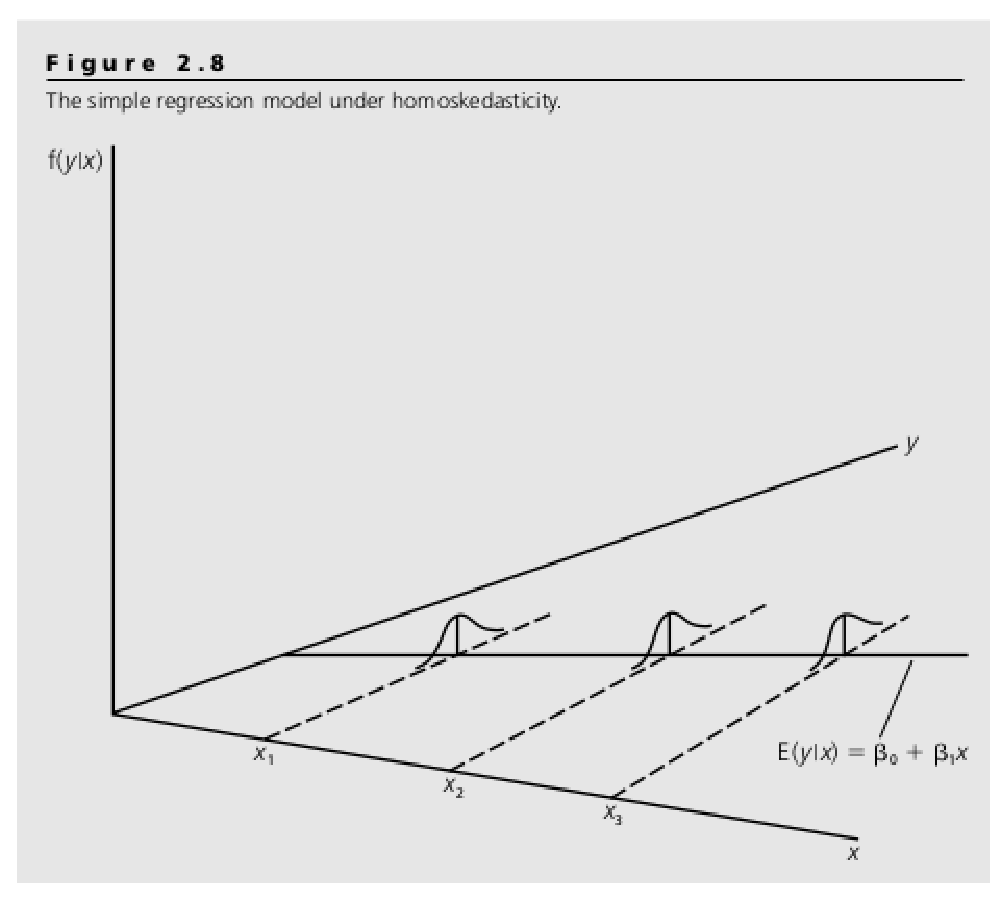
\includegraphics[scale = 0.5]{pictures/figure_2_8.eps}
\caption{Chybový člen vykazující homoskedasticitu}
\label{figure_2_6}
\end{figure} 

\begin{figure}[htp]
\centering
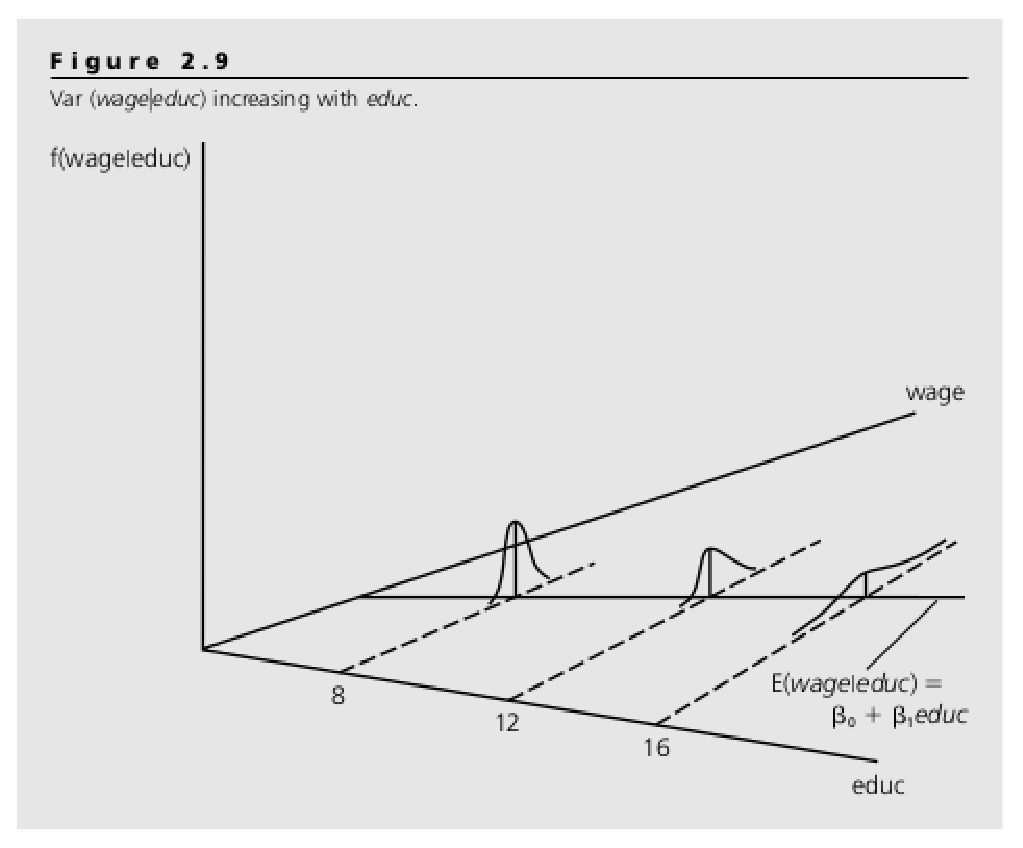
\includegraphics[scale = 0.5]{pictures/figure_2_9.eps}
\caption{Chybový člen vykazující heteroskedasticitu}
\label{figure_2_6}
\end{figure} 


\begin{theorem}
Při splnění předpokladů SLR.1 až SLR.5 platí
\begin{equation}
var[\hat{\beta}_1] = \frac{\sigma^2}{\sum_{i = 1}^n (x_i - \bar{x})^2} = \frac{\sigma^2}{SST_x}
\end{equation}
a
\begin{equation}
var[\hat{\beta}_0] = \frac{\sigma^2 \frac{1}{n}\sum_{i = 1}^n x_i^2}{\sum_{i = 1}^n (x_i - \bar{x})^2} = \frac{\sigma^2 
\frac{1}{n}\sum_{i = 1}^n x_i^2}{SST_x} = \frac{\sigma^2 \bar{x^2}}{SST_x}.
\end{equation}

\raggedleft{$\clubsuit$}
\end{theorem}

\begin{proof}
Nejprve odvoďme rozptyl $\hat{\beta}_1$. Výchozím bodem je rovnice (2.38), tj. $\hat{\beta}_1 = \beta_1 + \frac{1}{SST_x}\sum_{i = 1}^n d_i u_i$. Protože $\beta_1$ je 
konstanta, a protože podmiňujeme na $x_i$, jsou $SST_x$ a $x_i - \bar{x}$ nenáhodné. Vzhledem k tomu, že z důvodu 
náhodného výběru je $u_i$ nezávislé napříč $i$, je rozptyl součtu $u_i$ součtem rozptylu $u_i$.
\begin{multline}
var(\hat{\beta}_1) = \left(\frac{1}{SST_x}\right)^2 var\left[\sum_{i = 1}^n d_i u_i \right] = 
\left(\frac{1}{SST_x}\right)^2 \left(\sum_{i = 1}^n d_i^2 var[u_i] \right)\\
= \left(\frac{1}{SST_x}\right)^2 \left(\sum_{i = 1}^n d_i^2 \sigma^2 \right) = \sigma^2 \left(\frac{1}{SST_x}\right)^2 
\left(\sum_{i = 1}^n d_i^2 \right) = \frac{\sigma^2}{SST_x}
\end{multline}

Analogicky lze dovodit $var[\hat{\beta}_0]$, kdy vycházíme z rovnice (2.42).
\begin{multline}
var[\hat{\beta}_0] = var[\beta_0] + var[\beta_1 - \hat{\beta}_1]\bar{x}^2 + var[\bar{u}] = \frac{\sigma^2}{n} - var[\beta_1]\bar{x}^2\\
= \frac{\sigma^2}{n} - \frac{\sigma^2 \bar{x}^2}{SST_x} = \frac{\sigma^2}{n} - \frac{\sigma^2 (\frac{SST_x}{n} - 
\bar{x^2})}{SST_x} = \frac{\sigma^2 \bar{x^2}}{SST_x}
\end{multline}

\raggedleft{$\clubsuit$}
\end{proof}

S rostoucím rozptylem chyby $u$ roste $var[\hat{\beta}_0]$ a $var[\hat{\beta}_1]$; větší rozptyl z titulu 
nepozorovaných veličin, které jsou obsaženy v $u$ a které ovlivňují $y$, činí odhad $\beta_0$ a $\beta_1$ obtížnějším. 
Na druhou stranu větší rozptyl $x$ snižuje $var[\hat{\beta}_0]$ a $var[\hat{\beta}_1]$, protože variabilita $x$ 
usnadňuje kvantifikaci vztahu mezi $E[y|x]$ a $x$. Vzhledem ke jmenovateli v (2.46) a (2.47) je tak vhodné odhadovat $\beta_0$ a $\beta_1$ pro data, kde $\bar{x} = 0$, 
neboť $\sum_{i = 1}^n x_i^2 \ge \sum_{i = 1}^n (x_i - \bar{x})^2$. Dále také platí, že s tím, jak roste velikost náhodného výběru, se 
zvyšuje celkový rozptyl $x$. Proto větší náhodný výběr implikuje menší $var[\hat{\beta}_0]$ a $var[\hat{\beta}_1]$.

\subsection{Odhad rozptylu chybového členu}

Rovnice (2.46) a (2.47) nám umožňují kvantifikovat rozptyl odhadů $\hat{\beta}_0$ a $\hat{\beta}_1$ za 
předpokladu, že známe $\sigma^2$. V praxi však $\sigma^2$ zpravidla neznáme, a proto je ho třeba nahradit 
odhadem. Připomeňme, že $\sigma^2$ je rozptylem chyby $u$. Pro odhad $\sigma^2$ tedy využijeme výběrový rozptyl 
reziduí $\hat{u}_i$. Logickou volbou by se zdál odhad
\begin{equation}
\hat{\sigma}_2 = \frac{1}{n} \sum_{i = 1}^n u_i^2 = \frac{1}{n} SSR.
\end{equation}
Tento odhad však ignoruje dvě omezení, která musí splňovat OLS rezidua, a to $\sum_{i = 1}^n \hat{u}_i = 0$ a 
$\sum_{i = 1}^n x_i \hat{u}_i = 0$. Správná verze odhadu je tak
\begin{equation}
\hat{\sigma}_2 = \frac{1}{n-2}\sum_{i = 1}^n \hat{u}_i^2 = \frac{1}{n - 2}SSR.
\end{equation}

\begin{theorem}[Nestrannost odhadu $\sigma^2$]
Při splnění předpokladů SLR.1 až SLR.5 platí
\begin{equation}
E[\hat{\sigma}_2] = \sigma^2.
\end{equation}

\raggedleft{$\clubsuit$}
\end{theorem}

\begin{proof}
Rezidua $\hat{u}_i$ lze zapsat jako funkci chyb $u_i$.
\begin{multline}
\hat{u}_i = y_i - \hat{y}_i = (\beta_0 + \beta_1 x_i + u_i) - (\hat{\beta}_0 - \hat{\beta}_1x_i)\\
= u_i - (\hat{\beta}_0 - \beta_0) - (\hat{\beta}_1 - \beta_1)x_i.
\end{multline}
Pokud obě strany této rovnice vyjádříme ve střední hodnotě, získáme
\begin{equation}
0 = \bar{u} - (\hat{\beta}_0 - \beta_0) - (\hat{\beta}_1 - \beta_1)\bar{x}.
\end{equation}
Odečtením této rovnice od původní rovnice $\hat{u}_1 = u_i - (\hat{\beta}_0 - \beta_0) - 
(\hat{\beta}_1 - \beta_1)x_i$ získáme
\begin{equation}
\hat{u}_i = (u_i - \bar{u}) - (\hat{\beta}_1 - \beta_1)(x_i - \bar{x}).
\end{equation}
Proto platí
\begin{equation}
\hat{u}_i^2 = (u_i - \bar{u})^2 + (\hat{\beta}_1 - \beta_1)^2(x_i - \bar{x})^2 - 2(u_i - \bar{u})(\hat{\beta}_1 - 
\beta_1)(x_i - \bar{x}).
\end{equation}
Součtem přes všechna $i$ pak dostaneme
\begin{equation}
\sum_{i = 1}^n \hat{u}_i^2 = \sum_{i = 1}^n (u_i - \bar{u})^2 + (\hat{\beta}_1 - \beta_1)^2 \sum_{i = 1}^n (x_i - \bar{x}) - 2(\hat{\beta}_1 - 
\beta_1)\sum_{i = 1}^n u_i(x_i - \bar{x}).
\end{equation}
Očekávaná hodnota prvního členu je $(n - 1)\sigma^2$. Očekávaná hodnota druhého členu je $\sigma^2$, protože 
$E[(\hat{\beta}_1 - \beta_1)^2] = var[\hat{\beta}_1] = \sigma^2/S_x^2$. A konečně třetí 
člen lze vyjádřit jako $2(\hat{\beta}_1 - \beta_1)^2 S_x^2$, což v očekávané hodnotě odpovídá $2\sigma^2$. 
Spojením všech tří členů pak získáváme
\begin{equation}
E\left[\sum_{i = 1}^n \hat{u}_i^2 \right] = (n - 1)\sigma^2 + \sigma^2 - 2 \sigma^2 = (n - 2)\sigma^2
\end{equation}
neboli
\begin{equation}
E\left[\frac{SSR}{n-2}\right] = \sigma^2.
\end{equation}

\raggedleft{$\clubsuit$}
\end{proof}

$\hat{\sigma} = \sqrt{\hat{\sigma}^2}$ nazýváme standardní směrodatnou odchylkou regrese (SER - standard error of 
regression). Ačkoliv $\hat{\sigma}$ není nestranným odhadem $\sigma$, lze dokázat, že se jedná o konzistentní 
odhad $\sigma$, a proto našim účelům dobře poslouží. Odhad směrodatné odchylky $\hat{\beta}_1$ je tak roven
\begin{equation}
se(\hat{\beta}_1) = \frac{\hat{\sigma}}{\sqrt{SST_x}} = \frac{\hat{\sigma}}{\sqrt{\sum_{i = 1}^n (x_i - \bar{x})^2}}.
\end{equation}
Podobně směrodatnou odchylku odhadu $\hat{\beta}_0$ lze získat z $sd(\hat{\beta}_0)$ nahrazením $\sigma$ jeho 
odhadem $\hat{\sigma}$.

\subsection{Regresní model bez průsečíku}

Uvažujme regresní model
\begin{equation}
y = \beta_1 x + u.
\end{equation}
Odhad sklonu regresního modelu bez průsečíku je dán rovnicí
\begin{equation}
\tilde{\beta}_1 = \frac{\sum_{i = 1}^n x_i y_i}{\sum_{i = 1}^n x_i^2}.
\end{equation}
Pokud $\bar{x} = 0$, pak $\hat{\beta}_1 = \tilde{\beta}_1$.

\section{Dodatek 2A}

\subsection{Metoda nejmenších čtverců}

Z předchozího textu víme, že
\begin{equation}
\hat{u}_i = y_i - \hat{y}_i = y_i - \hat{\beta}_0 - \hat{\beta}_1 x.
\end{equation}
Definujme
\begin{equation}
Q(b_0, b_1) = \sum_{i = 1}^n (y_i - b_0 - b_1 x_i)^2,
\end{equation}
kde $b_0$ a $b_1$ jsou fiktivní proměnné pro účely definice optimalizačního problému. Hodnoty $b_0$ a $b_1$, které minimalizují $Q(b_0, b_1)$, lze získat 
řešením soustavy rovnic $\frac{\partial Q(b_0, b_1)}{\partial b_0} = 0$ a $\frac{\partial Q(b_0, b_1)}{b_1} = 0$, tj.
\begin{equation}
-2 \sum_{i = 1}^n (y_i - b_0 - b_1 x_i) = 0
\end{equation}
a
\begin{equation}
-2 \sum_{i = 1}^n x_i(y_i - b_0 - b_1 x_i) = 0.
\end{equation}
S pomocí první derivace lze nalézt extrém funkce, nikoliv však nutně její minimum. To, že $b_0$ a $b_1$ 
skutečně minimalizují hodnotu $Q(b_0, b_1)$, lze ověřit následujícím způsobem.
\begin{multline}
Q(b_0, b_1) = \sum_{i = 1}^n \left[y_i - \hat{\beta}_0 - \hat{\beta}_1 x_i + (\hat{\beta}_0 - b_0) + (\hat{\beta}_1 - 
b_1) x_1 \right]^2\\
= \sum_{i = 1}^n \left[\hat{u}_i + (\beta_0 - b_0) + (\hat{\beta}_1 - b_1)x_i \right]^2\\
= \sum_{i = 1}^n \hat{u}_i^2 + n(\hat{\beta}_0 - b_0)^2 + (\hat{\beta}_1 - b_1)^2 \sum_{i = 1}^n x_i^2 + 
2(\hat{\beta}_0 - b_0)(\hat{\beta}_1 - b_1)\sum_{i = 1}^n x_i
\end{multline}
První člen nezávisí na $b_0$ a $b_1$ a zbývající tři členy lze přepsat do tvaru $\sum_{i = 1}^n 
\left[(\hat{\beta}_0 - b_0) + (\hat{\beta}_1 - b_1)x_i \right]^2$, který může být nejméně roven nule, což 
nastává právě pro $b_0 - \hat{\beta}_0$ a $b_1 = \hat{\beta}_1$.
